\documentclass{article}

\usepackage[utf8]{inputenc}
\usepackage[brazilian]{babel}
\usepackage{graphicx}
\usepackage{float}
\usepackage[pdftex]{hyperref}
\usepackage{epstopdf}
\usepackage{etoolbox}
\usepackage{amsmath}
\usepackage{amsfonts}
\usepackage{amssymb}
\usepackage{caption}
\usepackage{subcaption}
\usepackage{setspace}
\usepackage{tikz}
\usepackage{listings}
\usepackage{xcolor} 

\patchcmd{\thebibliography}{\section*}{\section}{}{}
\newcommand{\R}{\ensuremath{\mathbb{R}}}
\newcommand{\Prob}{\ensuremath{\mathbb{P}}}
\newcommand{\K}{\ensuremath{\mathbb{K}}}
\newcommand{\U}{\ensuremath{\mathbb{U}}}
\newcommand{\N}{\ensuremath{\mathbb{N}}}
\newcommand{\Lg}{\ensuremath{\mathbb{L}}}
\newcommand{\T}{\ensuremath{\rm Tr}}
\newcommand{\sg}{{\sigma(x_k)}}

\newcommand{\G}{\ensuremath{\mathcal{G}}}
\newcommand{\F}{\ensuremath{\mathcal{F}}}
\newcommand{\C}{\ensuremath{\mathcal{C}}}
\newcommand{\E}{\ensuremath{\mathcal{E}}}
\newcommand{\Hn}{\ensuremath{\mathcal{H}}}
%\newcommand{\Hoo}{\ensuremath{\mathcal{H}_\infty}}
\newcommand{\Hop}{\ensuremath{\mathcal{H}_{op}}}
% --------------------------------------------------
\newtheorem{theo}{Teorema}
\newtheorem{exa}{Exemplo}
\newtheorem{lemm}{Lema}
\newtheorem{coro}{Corolário}
\newtheorem{defn}{Definição}[section]

%opening
\lstset{ %
	backgroundcolor=\color{black},   % choose the background color; you must add \usepackage{color} or \usepackage{xcolor}
	basicstyle=\footnotesize,        % the size of the fonts that are used for the code
	breakatwhitespace=false,         % sets if automatic breaks should only happen at whitespace
	breaklines=true,                 % sets automatic line breaking
	captionpos=t,                    % sets the caption-position to bottom
	commentstyle=\color{green},    % comment style
	extendedchars=true,              % lets you use non-ASCII characters; for 8-bits encodings only, does not work with UTF-8
	frame=single,                    % adds a frame around the code
	keepspaces=true,                 % keeps spaces in text, useful for keeping indentation of code (possibly needs columns=flexible)
	keywordstyle=\color{cyan},       % keyword style
	language=C,                 % the language of the code
	numbers=left,                    % where to put the line-numbers; possible values are (none, left, right)
	numbersep=5pt,                   % how far the line-numbers are from the code
	numberstyle=\tiny\color{black}, % the style that is used for the line-numbers
	rulecolor=\color{gray},         % if not set, the frame-color may be changed on line-breaks within not-black text (e.g. comments (green here))
	showspaces=false,                % show spaces everywhere adding particular underscores; it overrides 'showstringspaces'
	showstringspaces=false,          % underline spaces within strings only
	showtabs=false,                  % show tabs within strings adding particular underscores
	stepnumber=2,                    % the step between two line-numbers. If it's 1, each line will be numbered
	stringstyle=\color{red},     % string literal style
	tabsize=2,                       % sets default tabsize to 2 spaces
	basicstyle=\color{orange}
}


\begin{document}

\begin{titlepage}
\begin{center}

\newcommand{\HRule}{\rule{\linewidth}{0.5mm}}
% Upper part of the page. The '~' is needed because \\
% only works if a paragraph has started.

\includegraphics[width=0.15\textwidth]{logoUnicamp}~\\[1cm]

\textsc{\LARGE Universidade Estadual de Campinas}\\[1.5cm]

\textsc{\Large Faculdade de Engenharia Mecânica}\\[0.5cm]

% Title
\HRule \\[0.4cm]
{ \huge \bfseries ES670 - Projeto de Sistemas Embarcados\\ \vspace{1cm} Relatório - Projeto Prático (Parte 1/7) \\
\Large{Requisitos de Teclado, LEDs e Display de Sete Segmentos} \\[0.4cm] }

\HRule \\[1.5cm]

% Author and supervisor
\begin{minipage}{0.6\textwidth}
\begin{flushleft} \large
\emph{Nome:}\\
Rodolfo Nobre Bitu de Morais\\Guilherme de Oliveira Souza\\ Marcelli Tiemi Kian
\end{flushleft}
\end{minipage}
\begin{minipage}{0.2\textwidth}
\begin{flushright} \large
\emph{RA}\\ 105654\\117093\\
117892
\end{flushright}
\end{minipage}

\vfill

% Bottom of the page
{\large \today}

\end{center}
\end{titlepage}


\onehalfspacing
\section{Objetivo} 
O objetivo do projeto é, de maneira incremental, implementar no target os requisitos apresentados no roteiro\cite{bb:roteiro} inicialmente desenvolvendo o modelo e depois implementando cada requisito. Estes requisitos são referentes à configuração e implementação de entradas de teclado, acionamento de LEDs, display de sete segmentos, protocolo de comunicação, display LCD, medição de velocidade de rotação, PWM, ADC e Controlador. 
	
\section{Modelagem}
% Diagramas requisitos implementados, digrama de blocos, etc
Utilizando o Rational Rhapsody Modeler e tomando como base os requisitos propostos mostrados na figura \ref{fig:requisitos}, complementamos o modelo inicial\cite{bb:modelo} (requisitos de teclado e LEDs) adicionando um bloco ao modelo referente aos displays de sete segmentos (REQ1C), conforme mostrado na figura \ref{fig:blocos}.

\begin{figure}[H]
	\centering
	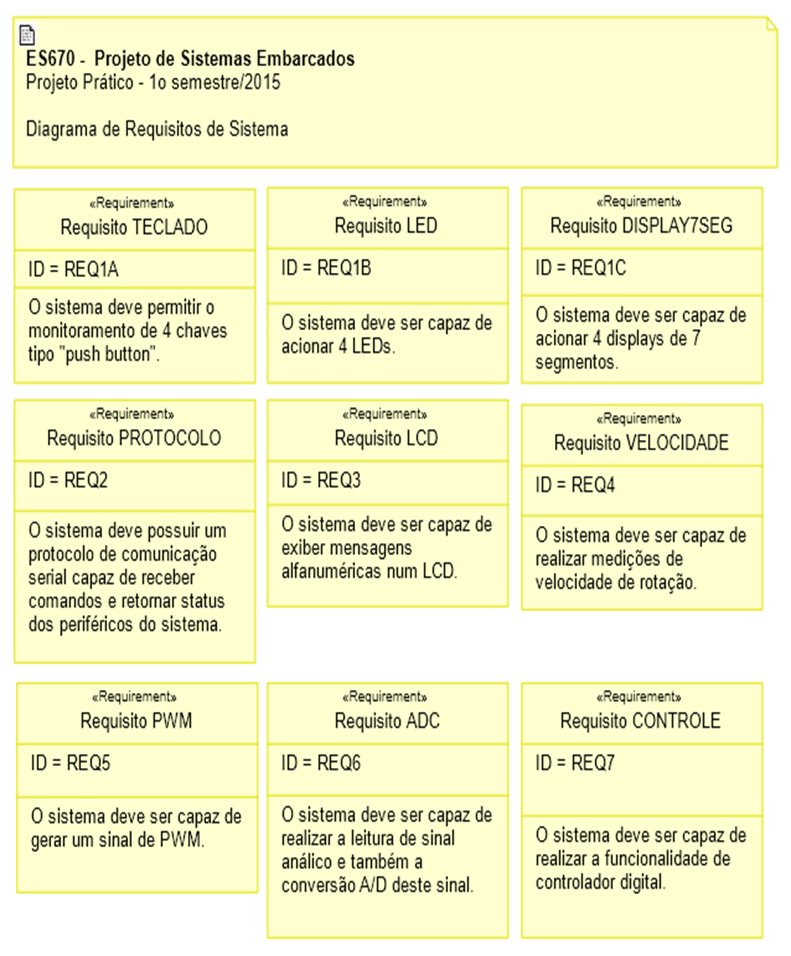
\includegraphics[width=0.9\linewidth]{requisitos}
	\caption{Diagrama de requisitos}
	\label{fig:requisitos}
\end{figure}
\begin{figure}[H]
	\centering
	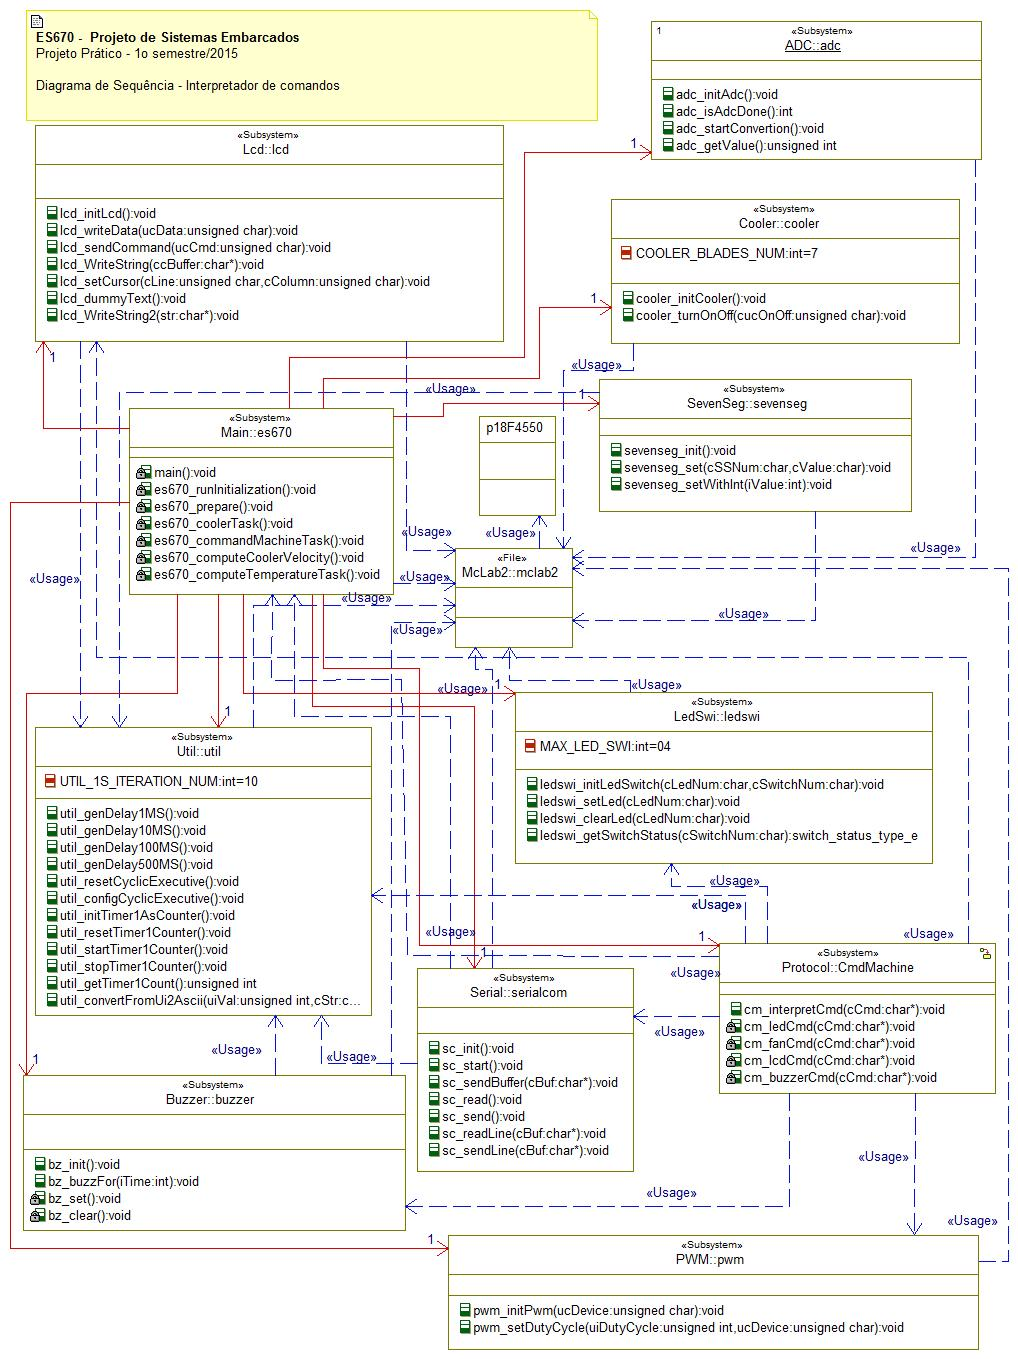
\includegraphics[width=0.9\linewidth]{blocos}
	\caption{Diagrama de definição de blocos}
	\label{fig:blocos}
\end{figure}
O bloco "SevenSeg" possui três operações: inicialização, definição de saída (recebendo qual dos displays será usado e qual valor deve ser exibido) e definição de saída com inteiro (recebendo apenas o valor inteiro a ser exibido no conjunto de quatro displays).

Com o objetivo de cumprir o requisito de comunicação serial (REQ2), foram adiconados os blocos Serial e CmdMachine. O bloco "Serial" é o bloco responsável pela comunicação serial simples, tendo como funções mandar e receber as mensagens. O bloco "CmdMachine" já tem a função de interpretar o que é recebido pela porta serial.

\section{Diagramas Esquemáticos}
% Diagramas esquemáticos do target utilizados

\begin{figure}[H]
	\centering
	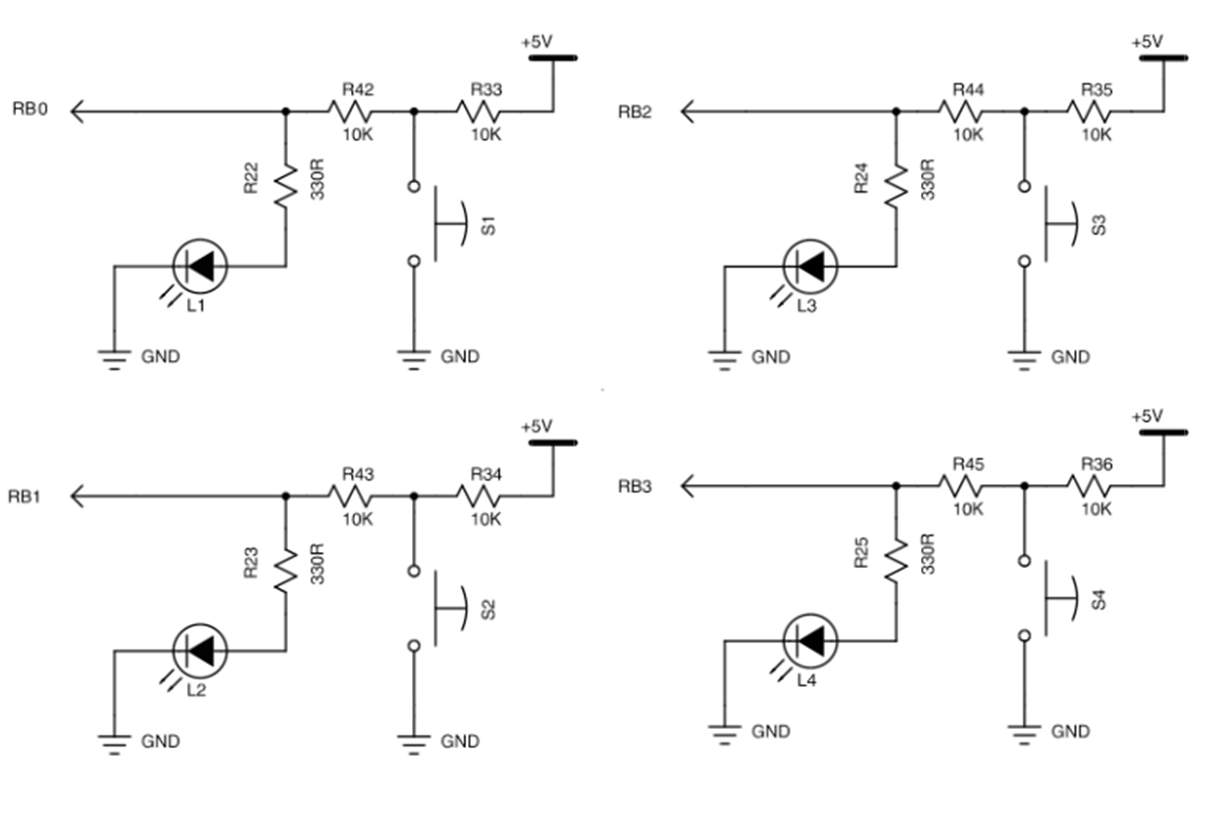
\includegraphics[width=0.7\linewidth]{esq_ledswi}
	\caption{Esquema teclado e LEDs}
	\label{fig:esq_ledswi}
\end{figure}
\begin{figure}[H]
	\centering
	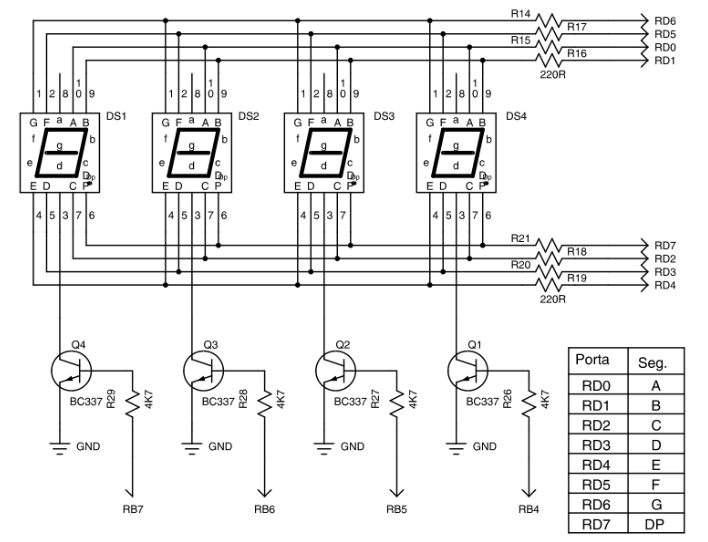
\includegraphics[width=0.9\linewidth]{esq_7seg}
	\caption{Esquema sete segmentos}
	\label{fig:esq_7seg}
\end{figure}
\begin{figure}[H]
	\centering
	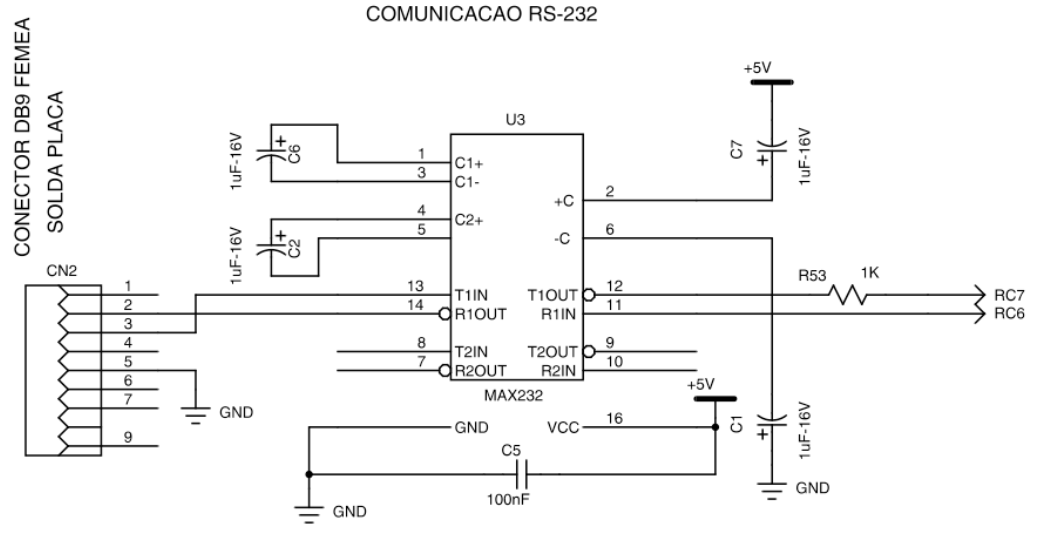
\includegraphics[width=0.9\linewidth]{serial}
	\caption{Esquema comunicação serial}
	\label{fig:serial}
\end{figure}

Como pode ser visto na figura \ref{fig:esq_7seg}, é necessário fazer um gerenciamento das portas RB4-7 e RD0-7 para que sejam mostrados os valores desejados nos displays de sete segmentos. Para isso, é preciso alternar qual RB está ativo fazendo a mudança nos RD0-7 para que cada display esteja mostrando um valor diferente. É importante lembrar que a frequência dessa alternância seja escolhida de modo que o olho humano não perceba que os displays estão ligando e desligando.

Observando a figura \ref{fig:serial}, para a manipulação da comunicação serial é necessário fazer a configuração inicial das portas TXSTA, RCSTA e BAUDCON e dos bits RC7 e RC6 para que a comunicação serial funcione da forma apropriada para nossa utilização.  Para enviar atravez da porta serial, é necessário que o bit TXIF da porta PIR1 esteja TRUE e colocar o que será enviado em TXREG. Para receber, é necessario que o bit RCIF da porta PIR1 esteja TRUE e ler RCREG.

\section{Implementação da sintaxe do protocolo de comunicação}

Após a leitura dos dados recebidos pela funçao ``sc\_receiveBuffer", o comando é interpretado pela função ``cm\_interpretCmd'' e então é executado um deternimado comportamento.

A sintaxe para comunicação é definida como:
\begin{itemize}
\item L[CS][1-4] - Comanda um led [1-4] para ligar ou desligar [CS], onde C é clear e S é set.
\item S[1-4] - Retorna o estado do switch [1-4]. A resposta é dada como aberta ou fechada [OC], onde O é opened e C é closed.
\item Bx - Onde x é um inteiro, comanda o buzzer para ligar durante x milesegundos.
\end{itemize}


\section{Matriz de Rastreabilidade}
% Matriz de rastreabilidade de requisitos vs implementações
A matriz de rastreabilidade apresentada na tabela \ref*{tab:rastreabilidade} relaciona cada um dos requisitos com a sua implementação.
\begin{table}[H]
	\centering
	\caption{Matriz de Rastreabilidade}
	\label{tab:rastreabilidade}
	\small
	\begin{tabular}{|c|l|}
		\hline \bfseries{ID do Requisito} & \bfseries{Implementação}\\ 
		\hline REQ1A 	& \texttt{ledswi.c}\\ 
						& \texttt{- void ledswi\_initLedSwitch(char cLedNum, char cSwitchNum)}\\
						& \texttt{- switch\_status\_type\_e ledswi\_getSwitchStatus(char cSwitchNum)}\\
		\hline REQ1B 	& \texttt{ledswi.c}\\ 
						& \texttt{- void ledswi\_initLedSwitch(char cLedNum, char cSwitchNum)}\\
						& \texttt{- void ledswi\_setLed(char cLedNum)}\\ 
						& \texttt{- void ledswi\_clearLed(char cLedNum)}\\
		\hline REQ1C 	& \texttt{sevenSeg.c}\\ 
						& \texttt{- void sevenseg\_init(void)}\\
						& \texttt{- void sevenseg\_set(char cSSNum, sevenseg\_value\_e eValue)}\\
						& \texttt{- void sevenseg\_setWithInt (int iValue)}\\
		\hline REQ2	 	& \texttt{serialcom.c}\\ 
						& \texttt{- void sc\_init(void)}\\
						& \texttt{- void sc\_start(void)}\\
						& \texttt{- void sc\_sendBuffer(char cBuf[])}\\
						& \texttt{- void sc\_receiveBuffer(char cBuf[])}\\
					& \texttt{cmdMachine.c}\\ 
						& \texttt{- void cm\_interpretCmd(char cCmd[]);}\\
		\hline 
	\end{tabular} 
	\normalsize
\end{table}
\section{Notas}
% Dificuldades, observações relevantes, correções, ...
Os maiores problemas identificados foram a dificuldade de conseguir conectar a placa com o computador e alguns mal contatos relacionados aos botões e do próprio PIC. Além disso, houve alguns conflitos com a IDE, pois muitas funcionalidades poderiam ter sido implementadas, já que a função de auto-completar é bem comum em IDE's e o duplo clique poderia selecionar a palavra em vez de colocar um breakpoint.


\begin{thebibliography}{widestlabel}
	\bibitem{bb:roteiro}{Roteiro de Laboratório - Semanas 04 e 05 (disponibilizado para os alunos)}
	\bibitem{bb:modelo}{Projeto do Modelo Inicial do Sistema (disponibilizado para os alunos)}
	\bibitem{bb:codigo}{Código Fonte Inicial em Linguagem C (disponibilizado para os alunos)}
\end{thebibliography}

\section{Apêndice}
% Colocar como apêndice toda a listagem do código fonte
Listagem dos códigos fonte:
\lstinputlisting[language=C, title = \lstname]{../headers/ledswi.h}
\lstinputlisting[language=C, title = \lstname]{../src/ledswi.c}
\lstinputlisting[language=C, title = \lstname]{../headers/es670_pp.h}
\lstinputlisting[language=C, title = \lstname]{../src/es670_pp.c}
\lstinputlisting[language=C, title = \lstname]{../headers/mclab2.h}
\lstinputlisting[language=C, title = \lstname]{../headers/util.h}
\lstinputlisting[language=C, title = \lstname]{../src/util.c}
\lstinputlisting[language=C, title = \lstname]{../headers/sevenSeg.h}
\lstinputlisting[language=C, title = \lstname]{../src/sevenSeg.c}
\end{document}

